\section{The Support Vector Machine (SVM)}

\mode<presentation>{
\begin{frame} 
    \begin{center} \huge
        \secname
    \end{center}
    \begin{center}
     Finding the separating hyperplane with maximum margin\\+ the ``kernel trick''   
    \end{center}
\end{frame}
}

\subsection{SVMs are Maximum Margin Classifiers}

\begin{frame}\frametitle{The binary classification setting}

\mode<article>{
The binary classification setting:\\

\begin{figure}[h]
    \centering
    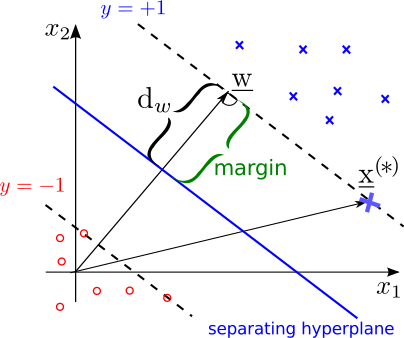
\includegraphics[height=4cm]{img/section2_fig13_v2_space} 
    \mode<article>{
    \caption{
    Binary classification setting.
    }
    \label{fig:setting}
    } 
\end{figure}
}
\mode<presentation>{
\placeimage{8.7}{2.2}{img/section2_fig13_v2_space}{width=4.8cm}
}


\begin{itemize}
	\item \underline{Data}:\\
    
	$
	\Big\{ \left(\vec x^{(\alpha)}, y^{(\alpha)}_{T} \right) \Big\}_{\alpha=1}^{p}\,
	$\\
	where $\vec x \in \R^{N}$, $y_T \in \{-1, 1\}$\\

	\item \underline{Model}:\\
    
	$
	y(\vec x; \vec w,b) = \sign \big( \vec w^{\top} \vec x + b \big)
	$
    
    \item \underline{Objective}:
    
    Choose the decision boundary s.t. the margin is \emph{maximal}.
    
    \item \underline{Assumption}:
    
    Perfect linear separation of both classes.
    
    \pause
    
    In the case of a simple connectionist neuron:
    \begin{equation}
    \vec w^{\top} \vec x + b \;\;
    \left \{ \begin{array}{ll}
					\ge& 0 \;\;\text{for } {\color{blue}y_{T} = +1}\\
					<& 0 \;\;\text{for } {\color{red}y_{T} = -1}
				\end{array} \right.  
    \end{equation}
    The solution here is not unique.
    
\end{itemize}
    
\end{frame}

\begin{frame}\frametitle{\subsecname}
    \mode<presentation>{
\placeimage{8.7}{2.4}{img/section2_fig13_v2_space}{width=5.5cm}
}
\begin{minipage}{6cm}
Let $\vec w^{*}$ and $b^{*}$ describe the optimal hyperplane that maximizes the margin of separation:
    \begin{equation}
    \vec w^{*\top} \vec x + b^{*} \;\;
    \left \{ \begin{array}{lll}
					\ge& 1 \;&\text{for } {\color{blue}y_{T} = +1}\\
					\le& -1 \;&\text{for } {\color{red}y_{T} = -1}
				\end{array} \right.  
    \end{equation}
    
    Points that lie on the margin are characterized by:
    
    \slidesonly{\vspace{-3mm}}
    
    \begin{equation}
    \vec w^{*\top} \vec x + b^{*} \;\;
    \left \{ \begin{array}{lll}
					=& 1 \;&\text{for } {\color{blue}y_{T} = +1}\\
					=& -1 \;&\text{for } {\color{red}y_{T} = -1}
				\end{array} \right.
			\quad \longleftarrow\; \text{``support vectors''} 
    \end{equation}
    
       

\end{minipage}\\
  
   \notesonly{
    These points will be referred to as the \emph{support vectors}.
    The shortest distance between points with opposite class labels is $2 \mathrm{d}_{w} = \frac{2}{\lVert \vec w^{*} \rVert}_{2}$, i.e. the distance separating the two classes.
    }
    
    \slidesonly{\vspace{3mm}}
    
    Maximizing the margin $\corresponds$ minimizing the Euclidean norm of $\vec w$.
    
    
    \begin{equation}
    \mathrm{d}_{w} = \frac{1}{\lVert \vec w \rVert_2} \eqexcl \max 
    \quad \corresponds \quad 
    \lVert \vec w \rVert_2 \eqexcl \min
    \end{equation}
    
    
    The solution to this is unique.

\end{frame}

\begin{frame}\frametitle{structural risk minimization (SRM) applied to binary classification}


The cost function\notesonly{ to minimize}:

\slidesonly{\vspace{-7mm}}
    
\begin{equation}
\frac{1}{2} \vec w^{\top} \vec w = \frac{1}{2} \lVert \vec w \rVert_{2}^{2} \eqexcl \min    
\end{equation}

\question{Why have we suddenly switched to the squared Euclidean norm and where did the 2 come from?}

\mode<article>{
- Minimizing the square of the norm turns it into a \emph{convex} minimization problem, which simplifies the optimization procedure.
Dividing by 2 is simply for convenience.
}


\notesonly{
We want to restrict the space of solutions for $\vec w$ to that which leads to the correct classification of the training points.
We therefore constrain solutions such that:}

\slidesonly{Constraint for correct classification (``\emph{0-1 loss}'' or ``\emph{hinge loss}''):}

\slidesonly{\vspace{-2mm}}

\begin{equation}
 y_{T}^{(\alpha)} \cdot \big( \vec w^{\top} \vec x^{(\alpha)} + b \big) \ge 1 \;\;\forall \alpha{}
 \label{eq:constraint}
\end{equation}

\notesonly{
\eqref{eq:constraint} provides constraints that are linear in $\vec w$. It is sometimes referred to as the \emph{0-1 loss} or \emph{hinge loss}. It is exactly zero whenever a point is correctly classified and 1 whenever it is misclassified. It behaves similarly to \emph{parity-check} with the difference that \emph{parity-check} only produces a binary output.

This gives us the \emph{primal} problem for structural risk minimization (SRM) problem. }
\slidesonly{The SRM principle is about:}


\slidesonly{\vspace{-3mm}}

\begin{figure}[h]
	\slidesonly{
    %\raggedleft
    \centering
    }
	\notesonly{
    \centering
    }
    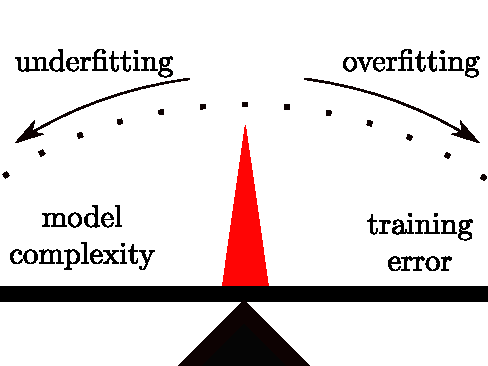
\includegraphics[height=3cm]{img/scale} 
    \mode<article>{
    \caption{
    The SRM principle is about balancing the complexity of a model while minimizing the training error to avoid overfitting.
    }
    }
\end{figure}
    
\end{frame}

\begin{frame}
Applying the Lagrange method to the primal problem of SRM:

\begin{equation}
f_{0}(\vec w,b) = \frac{1}{2} \lVert \vec w \rVert_{2}^{2} = \frac{1}{2} \vec w^{\top} \vec w \eqexcl \min
\end{equation}
\notesonly{
Manipulating the constraints \eqref{eq:constraint} to obtain an expression in the form $f_{\alpha} \le 0$:
}

A constraint $f_\alpha(\vec w,b) \le 0$ for each data point in the training set:

\pause

\slidesonly{\vspace{-3mm}}

\begin{align}
 y_{T}^{(\alpha)} \cdot \big( \vec w^{\top} \vec x^{(\alpha)} + b \big) \,\ge\, &1\\
 y_{T}^{(\alpha)} \cdot \big( \vec w^{\top} \vec x^{(\alpha)} + b \big) -1 \,{\color{blue}\ge}\, &0\\
 {\color{blue}-}\big\{y_{T}^{(\alpha)} \cdot \big( \vec w^{\top} \vec x^{(\alpha)} + b \big) -1\big\} \,{\color{blue}\le}\, &0
\end{align}

\begin{equation}
f_{\alpha} (\vec w,b) = -\big\{ y_{T}^{(\alpha)} \cdot \big( \vec w^{\top} \vec x^{(\alpha)} + b \big) -1 \big\} \le 0\;,\quad \alpha = 1,\ldots,p    
\end{equation}

The Lagrangian becomes:

\pause

\slidesonly{\vspace{-5mm}}

\begin{align}
L(\vec w, b, \{\lambda_{\alpha}\}) 
\,=&\, f_{0}(\vec w,b) + \sum_{\alpha=1}^{p} \lambda_{\alpha} f_{\alpha}(\vec w,b)\\
\,=&\, \frac{1}{2} \lVert \vec w \rVert_{2}^{2}
- \sum_{\alpha=1}^{p} \lambda_{\alpha} \big\{ y_{T}^{(\alpha)} \cdot \big( \vec w^{\top} \vec x^{(\alpha)} + b \big) -1 \big\}
\label{eq:lagrangianprimal}\slidesonly{,\quad \lambda_{\alpha} \ge 0}
\end{align}

\end{frame}

\begin{frame}

\mode<presentation>{
\vspace{-2mm}
\begin{block}{The Lagrangian of the primal problem:}
\vspace{-2mm}
	\begingroup 
	\footnotesize
\begin{equation*}
L(\vec w, b, \{\lambda_{\alpha}\}) = \frac{1}{2} \lVert \vec w \rVert_{2}^{2}
- \sum_{\alpha=1}^{p} \lambda_{\alpha} \big\{ y_{T}^{(\alpha)} \cdot \big( \vec w^{\top} \vec x^{(\alpha)} + b \big) -1 \big\}
,\quad \{\lambda_{a} \ge 0\}_{\alpha=1}^{p}
\end{equation*}
	\endgroup
\end{block}
}

\notesonly{where $\{\lambda_{a} \ge 0\}_{\alpha=1}^{p}$ is the set of Lagrange multipliers. Because of the minus sign in front of the multipliers, t}\slidesonly{T}he Lagrangian is optimized by
\begin{itemize}
\item[] \emph{\textcolor{blue}{minimizing}} w.r.t. $\vec w$ and $b$, the \emph{``primal variables''}, and 
\item[] \emph{\textcolor{darkgreen}{maximizing}} w.r.t. all $\lambda_{\alpha}$, the \emph{``dual variables''}.
\end{itemize}

%\slidesonly{\vspace{5mm}}
This, along with the minimization being \emph{convex} and the constraints being linear, implies that a \emph{saddle point} has to be found for the Lagrangian.

\only<2>{
\begin{figure}[h]
    \centering
    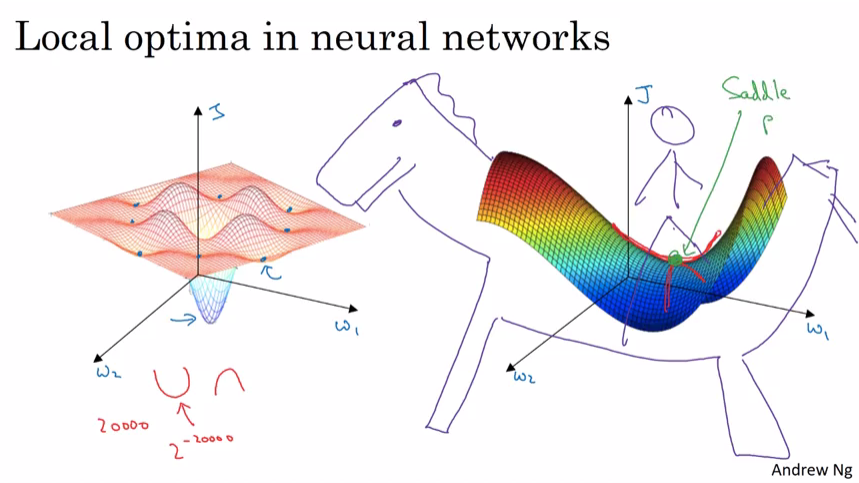
\includegraphics[trim={0cm 0 0 25mm},clip, height=4cm]{img/saddle_point_andrewng} 
    \mode<article>{
    \caption{
    Illustration of a saddle point.
    }
    \label{fig:saddle}
    } 
\end{figure}
}
\only<3>{
\slidesonly{\vspace{5mm}}

\begin{block}{Equivalent optimization problems (Kuhn and Tucker theorem):}

\begin{equation}
		{\color{blue}\min_{\vec w, b}}~L{(\vec{w}, b, {\color{darkgreen} \{ \lambda_\alpha^*\}})}
		= L{({\color{blue}\vec{w}^*}, {\color{blue}b^*}, {\color{darkgreen} \{ \lambda_\alpha^*\}})}
		= {\color{darkgreen}\max_{ \lambda_\alpha \geq 0}}~L{({\color{blue}\vec{w}^*}, {\color{blue}b^*}, \{ \lambda_\alpha \})}
\end{equation}

\end{block}
}

\end{frame}


\subsection{Karush-Kuhn-Tucker (KKT) conditions}

\begin{frame}\frametitle{\subsecname}

\question{What is happening as we optimize the Lagrangian of the primal problem?}


\mode<article>{
- We will attempt to answer this by looking at the constraints and how different cases for the constraints affect the Lagrangian and in turn the variables we are optimizing.
This will leads us to identifying the Karush-Kuhn-Tucker (KKT) conditions.
}

\end{frame}

\begin{frame}{Only}\frametitle{\subsecname}

\only<1-5>{
\slidesonly{\vspace{-3mm}}
\begin{block}{\notesonly{Recall}}

\begin{enumerate}
\item the constrained optimization problem:
\slidesonly{\vspace{-2mm}}

	\begingroup 
	\footnotesize
	\begin{equation*}
	\begin{array}{ll}
	\min_{\vec w, b} & \frac{1}{2} \lVert \vec w \rVert_{2}^{2}\\
	\text{subject to} & 
	-\big\{ y_{T}^{(\alpha)} \kern-.5ex \cdot \kern-.5ex \big( \vec w^{\top} \vec x^{(\alpha)} + b \big) -1 \big\} \le 0\;,\quad \text{for all } \alpha = 1,\ldots,p,
	\end{array}
	\end{equation*}
	\endgroup 

\item the corresponding Lagrangian:

	\slidesonly{\vspace{-3mm}}
	\begingroup 
	\footnotesize
	\begin{equation*}
		L(\vec w, b, \{\lambda_{\alpha}\}) = \frac{1}{2} \lVert \vec w \rVert_{2}^{2}
		- 
		\notesonly{\sum_{\alpha=1}^{p}}
		\slidesonly{
		\only<1,2>{\sum_{\alpha=1}^{p}}
		\only<3>{{\color{red}\sum_{\alpha=1}^{p}}}
		\only<4-5>{\sum_{\alpha=1}^{p}}
		}
			\lambda_{\alpha} \big\{ y_{T}^{(\alpha)} \kern-.5ex \cdot \kern-.5ex \big( \vec w^{\top} \vec x^{(\alpha)} + b \big) -1 \big\}
		,\;\; \lambda_{\alpha} \ge 0,
		%\label{eq:lagrangianprimal}
	\end{equation*}
	\endgroup

\item and the equivalent optimization problems:

	\slidesonly{\vspace{-3mm}}
	\begingroup 
	\footnotesize
	\begin{equation*}
			{\color{blue}\min_{\vec w, b}}~L{(\vec{w}, b, {\color{darkgreen} \{ \lambda_\alpha^*\}})}
			= L{({\color{blue}\vec{w}^*}, {\color{blue}b^*}, {\color{darkgreen} \{ \lambda_\alpha^*\}})}
			= {\color{darkgreen}\max_{ \lambda_\alpha \geq 0}}~L{({\color{blue}\vec{w}^*}, {\color{blue}b^*}, \{ \lambda_\alpha \})}.
	\end{equation*}
	\endgroup

\end{enumerate}

\end{block}%Recall
}

%\only<1->
{
Consider the following cases:

\begin{enumerate}[(a)]
	\item<only@2> \notesonly{Whenever }a constraint is \textcolor{orange}{violated},\slidesonly{\\} i.e.
	\begingroup 
	\footnotesize
	$
	-\big\{ y_{T}^{(\alpha)} \kern-.5ex \cdot \kern-.5ex \big( \vec w^{\top} \vec x^{(\alpha)} + b \big) -1 \big\}~{\color{orange}>}~0
	$
	\endgroup 
	
\mode<presentation>{
\only<2>{
\placeimage{13.2}{11}{img/section2_fig18_sv_nolambda_violate_within}{width=2cm}
\placeimage{9.7}{11}{img/section2_fig18_sv_nolambda_violate_misclassification}{width=2cm}

\begin{textblock}{5}(12,15)
\mbox{\tiny$-\{+1\cdot0.2-1\} = +0.8~{\color{orange}>}~0$}
\end{textblock}
\begin{textblock}{5}(8.5,10)
\mbox{\tiny$-\{+1\cdot(-11)-1\} = +12~{\color{orange}>}~0$}
\end{textblock}
}}
	\mode<article>{
\begin{figure}[ht]
     \centering
     \savebox{\imagebox}{
	 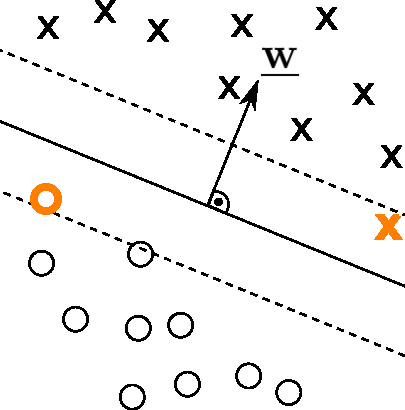
\includegraphics[width=0.22\textwidth]{img/section2_fig18_sv_nolambda_violate_within}}%
     \begin{subfigure}[t]{0.4\textwidth}
         \centering
         \usebox{\imagebox}% Place largest image
         \mode<article>{
         \caption{No points within the margin!}
         }
         \label{fig:violate_within_margin}
     \end{subfigure}
     \hspace{10mm}
     \begin{subfigure}[t]{0.3\textwidth}
         \centering
         \raisebox{\dimexpr.5\ht\imagebox-.5\height}{% Raise smaller image into place
         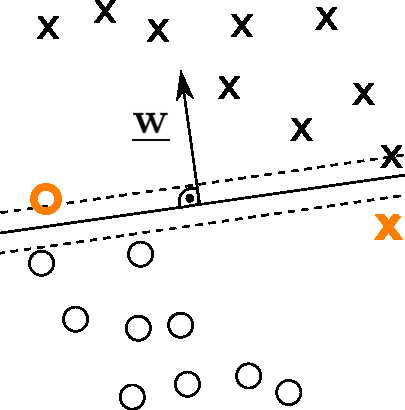
\includegraphics[width=0.77\textwidth]{img/section2_fig18_sv_nolambda_violate_misclassification}
         }
         \mode<article>{
         \caption{No misclassifications!}
         }
     \end{subfigure}
     \mode<article>{
     \caption{Possible causes of violating the constraint.}
	 }
	 \label{fig:violate}
\end{figure}
	}
	
	\notesonly{
	Increasing the value of the corresponding multiplier $\lambda_\alpha$ \emph{\textcolor{darkgreen}{increase}} $L$. 
	This will in turn lead to a change in the primal variables $\vec w$ and $b$ to \emph{\textcolor{blue}{decrease}} $L$.
	That is:
	}
	\begin{equation}
	\lambda_\alpha \uparrow \; \leadsto\quad L {\color{darkgreen}\uparrow} \; \leadsto \; \text{change in } \vec w,b \; \leadsto\; L {\color{blue}\downarrow}\slidesonly{\hspace{5cm}}
	\end{equation}
	
	% not really a case
	\item<only@3>[] \emph{\textcolor{blue}{Decrease}} of $L$ by changing $\vec w$ and $b$ prevents terms inside the \slidesonly{\only<3>{\textcolor{red}}{sum}} \notesonly{sum of the Lagrangian } from taking on arbitrarily large negative values.
	
	\item<only@4> Constraints are met but not \textbf{not} as equalities, i.e.
	\begingroup 
	\footnotesize
	$
	-\big\{ y_{T}^{(\alpha)} \cdot \big( \vec w^{\top} \vec x^{(\alpha)} + b \big) -1 \big\}~{\color{magenta}{<}}~0
	$\endgroup. \notesonly{$\lambda$'s are meant to maximize $L$. In this case, }\slidesonly{\\}$L$ can only be maximized by setting \notesonly{the corresponding multiplier }$\lambda_\alpha$ to zero.
	
	\mode<presentation>{
	\only<4>{
	\placeimage{12}{11}{img/section2_fig18_sv_legend_nolambda_met}{width=2.4cm}
		
	\begin{textblock}{5}(11,10.6)
	\mbox{\tiny$-\{-1\cdot(-11)-1\} = -10~{\color{magenta}<}~0$}
	\end{textblock}
	}
	}%presentation
	
	\item<only@5,6>  This leaves $\lambda_\alpha \ne 0$, which corresponds to the constraints being met with \emph{equality}, i.e. 
	\begingroup 
	\footnotesize
	$
	-\big\{ y_{T}^{(\alpha)} \cdot \big( \vec w^{\top} \vec x^{(\alpha)} + b \big) -1 \big\}~{\color{red}{\eqexcl}}~0
	$\endgroup. 

	\question{What does ``${\color{red}{=}} 0$'' imply w.r.t. misclassification?}\\

	\notesonly{
	-This implies that the choice of $\vec w$ and $b$ not only leads to correct classification of that training point but also that the point lies exactly on the margin, indicating that the point for which $\lambda_\alpha \ne 0$ is a \emph{support vector} (cf. \figref{fig:setting}). These are referred to as the \emph{Karush-Kuhn-Tucker (KKT) conditions}.
	}
	\only<6>{
	\begin{figure}[h]
		\centering
		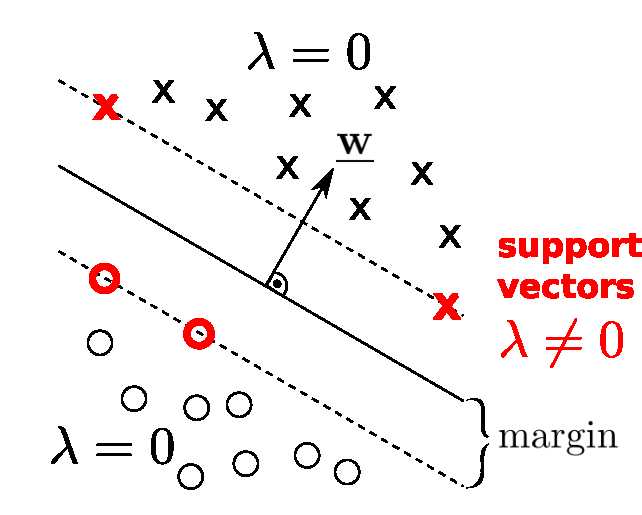
\includegraphics[height=4.5cm]{img/section2_fig18_sv} 
		\mode<article>{
		\caption{
		The constraint for support vectors is met with equality.
		}
		\label{fig:conditionsv}
		} 
	\end{figure}
	}
\end{enumerate}
}

\end{frame}

\begin{frame}\frametitle{\subsecname~Overview}
% Please add the following required packages to your document preamble:
% \usepackage[table,xcdraw]{xcolor}
% If you use beamer only pass "xcolor=table" option, i.e. \documentclass[xcolor=table]{beamer}

\begin{table}[h]
\notesonly{\hskip-2.0cm}% shift table to the left
\resizebox{\textwidth}{!}{%
\begin{tabular}{ccccll}
\begin{tabular}[c]{@{}c@{}}Where is\\ the point\\ relative to\\ the margin?\end{tabular} & \begin{tabular}[c]{@{}c@{}}label\\ $y_T$\end{tabular} & \begin{tabular}[c]{@{}c@{}}prediction\\ $\vec w^\top \vec x + b$\end{tabular} & \begin{tabular}[c]{@{}c@{}}correctly\\ classified\end{tabular} & \multicolumn{1}{c}{constraint value $f_{\alpha}$}      & \begin{tabular}[c]{@{}c@{}}constraint\\ met?\end{tabular}      
\\ \hline
outside  & $\mbox{\scriptsize+1}$                                                    & $\mbox{\scriptsize-11}$                                                        & no                                                             & $\mbox{\scriptsize-\{+1$\cdot$(-11) - 1\} = +12 > 0}$        & {\color[HTML]{F8A102} violated}
\\ \hline
outside  & $\mbox{\scriptsize-1}$                                                    & $\mbox{\scriptsize+30}$                                                         & no                                                             & $\mbox{\scriptsize-\{-1$\cdot$30 - 1\} = +31 > 0}$       & {\color[HTML]{F8A102} violated}
\\ \hline
inside   & $\mbox{\scriptsize+1}$                                & $\mbox{\scriptsize+0.2}$                                                        & yes                                                            & $\mbox{\scriptsize-\{+1$\cdot$0.2 - 1\} = +0.8 > 0}$        & {\color[HTML]{F8A102} violated}
\\ \hline
inside   & $\mbox{\scriptsize-1}$                                                   & $\mbox{\scriptsize-0.2}$                                                        & yes                                                            & $\mbox{\scriptsize-\{-1$\cdot$(-0.2) - 1\} = +0.8 > 0}$ & {\color[HTML]{F8A102} violated}
\\ \hline
outside  & $\mbox{\scriptsize+1}$                                                   & $\mbox{\scriptsize+200}$                                                        & yes                                                            & $\mbox{\scriptsize--\{+1$\cdot$200 - 1\} = -\{199\} < 0}$                & {\color[HTML]{DF02F8} met}
\\ \hline
outside  & $\mbox{\scriptsize-1}$                               & $\mbox{\scriptsize-10}$                                                         & yes                                                            & $\mbox{\scriptsize-\{-1(-10) - 1\} = -\{9\} < 0}$               & {\color[HTML]{DF02F8} met}
\\ \hline
on       & $\mbox{\scriptsize-1}$                                & $\mbox{\scriptsize-1}$                                                         & yes                                                            & $\mbox{\scriptsize-\{-1$\cdot$(-1) - 1\} = 0}$                              & \begin{tabular}[c]{@{}c@{}}{\color[HTML]{CB0000} met with}\\ {\color[HTML]{CB0000}equality}\end{tabular}
\end{tabular}
}
\caption{Example cases for the constraint.}
\end{table}
\end{frame}

\subsection{Solving the primal problem}

\begin{frame}\frametitle{\subsecname}

\mode<presentation>{
	\begingroup 
	\footnotesize
\begin{equation*}
L(\vec w, b, \{\lambda_{\alpha}\}) = \frac{1}{2} \lVert \vec w \rVert_{2}^{2}
- \sum_{\alpha=1}^{p} \lambda_{\alpha} \big\{ y_{T}^{(\alpha)} \cdot \big( \vec w^{\top} \vec x^{(\alpha)} + b \big) -1 \big\}
,\quad \lambda_{\alpha} \ge 0
\end{equation*}
	\endgroup
}

\notesonly{
The Lagrangian of the primal problem is solved by finding the saddle point.} At the saddle point, the derivatives of the Lagrangian $L$ w.r.t to the primal variables goes to zero:

\slidesonly{\vspace{-3mm}}

\begin{align}
\only<1,2>{
	\frac{\partial L}{\partial {w}_i} \;\eqexcl&\; 0 \quad \text{for } i=1,\ldots,N\\
	}
\only<2>{ 
	{w}_i - \sum\limits_{\alpha = 1}^p \lambda_\alpha
		y_T^{(\alpha)} \mathrm{x}_i^{(\alpha)} \;\eqexcl&\; 0 \\}
\only<3->{
		\Rightarrow\;\; \vec{w}^* =& \kern-4ex\underbrace{\sum_{\alpha = 1}^p \lambda_\alpha 
		y_T^{(\alpha)} \vec{x}^{(\alpha)}}_{
			\substack{	\text{expansion of the weight vector} \\
					\text{in terms of data points}}}	
					 \label{eq:primalsolution1}
}
\end{align}
\begin{align}
\only<3>{
	\frac{\partial L}{\partial b}
	= -\sum_{\alpha = 1}^p \lambda_\alpha y_T^{(\alpha)} &\eqexcl 0\\
	}
\only<4>{
	\sum_{\alpha = 1}^p \lambda_\alpha y_T^{(\alpha)} &\eqexcl 0
 \label{eq:primalsolution2}
	}
\end{align}

\only<4>{
The solution is unique for $\vec w$ but not for the set of multipliers $\{\lambda_{a}\}_{\alpha=1}^{p}$ (\notesonly{we haven't forgotten about $b^{*}$, }we will get to $b^{*}$ shortly).
}

\end{frame}

\subsection{From the primal problem to the dual problem}\label{sec:dualtoprimal}

\begin{frame}\frametitle{\subsecname}

\mode<presentation>{
\slidesonly{\vspace{-5mm}}
	\begingroup 
	\footnotesize
\begin{equation*}
L(\vec w, b, \{\lambda_{\alpha}\}) = \frac{1}{2} \lVert \vec w \rVert_{2}^{2}
- \sum_{\alpha=1}^{p} \lambda_{\alpha} \big\{ y_{T}^{(\alpha)} \cdot \big( \vec w^{\top} \vec x^{(\alpha)} + b \big) -1 \big\}
,\quad \lambda_{\alpha} \ge 0
\end{equation*}
	\endgroup
}
    
\begin{block}{The \emph{dual} problem:}
Solving the primal problem \slidesonly{(above)} in addition to finding a unique solution for the set of multipliers.
\end{block}

\pause 

\mode<presentation>{
Solution of the \emph{primal} problem:
\begin{align}
 \vec w^{*} &= \sum_{\alpha=1}^{p} \lambda_{\alpha} y_{T}^{(\alpha)} \vec x^{(\alpha)} &
 \label{eq:primalsolution1}
 &(1)
\intertext{and the condition}
 \sum_{\alpha=1}^{p} \lambda_{\alpha} y_{T}^{(\alpha)} &= 0& 
 \label{eq:primalsolution2} 
 &(2)
\end{align}
}

\eqref{eq:primalsolution1} and \eqref{eq:primalsolution2} are plugged back into the Lagrangian of the primal problem\notesonly{ \eqref{eq:lagrangianprimal}}.
\notesonly{From this follows:}

\end{frame}

\begin{frame}\frametitle{From the {primal} problem to the {dual} problem}

\mode<presentation>{
\vspace{-5mm}
\begingroup 
\footnotesize
\begin{equation}
(1)\quad
    \vec w^{*} = \sum_{\alpha=1}^{p} \lambda_{\alpha} y_{T}^{(\alpha)} \vec x^{(\alpha)}
%\label{eq:primalsolution1}
    \qquad\text{and}\qquad{}
(2)\quad 
    \sum_{\alpha=1}^{p} \lambda_{\alpha} y_{T}^{(\alpha)} = 0 
%\label{eq:primalsolution2} 
 \end{equation}
\endgroup
\vspace{-5mm}
}

\begingroup
\footnotesize
\begin{align}
\visible<1->{
\notesonly{
L(\vec w^*, b, &\{\lambda_{\alpha}\})\\}
\slidesonly{
L(\vec w^*, b, \{\lambda_{\alpha}\})}
=\,& \frac{1}{2} \vec w^{*\top} \vec w^{*}
- \sum_{\alpha=1}^{p} \lambda_{\alpha} \big\{ y_{T}^{(\alpha)} \cdot \big( \vec w^{*\top} \vec x^{(\alpha)} + b \big) -1 \big\}\\
}
\visible<2->{
=\,& \frac{1}{2} \vec w^{*\top} \vec w^{*}
-  \sum_{\alpha=1}^{p} \lambda_{\alpha} y_{T}^{(\alpha)} {\color{blue}\vec w^{*\top}} \vec x^{(\alpha)}
-  \sum_{\alpha=1}^{p} \lambda_{\alpha} y_{T}^{(\alpha)} {\color{blue}b}
+ \sum_{\alpha=1}^{p} \lambda_{\alpha}\\
}
\visible<3->{
=\,& \frac{1}{2} \vec w^{*\top} \vec w^{*}
- {\color{blue}\vec w^{*\top}} \underbrace{\sum_{\alpha=1}^{p} \lambda_{\alpha} y_{T}^{(\alpha)} \vec x^{(\alpha)}}_{= \vec w^* \text{ (cf. \eqref{eq:primalsolution1})}}
- {\color{blue}b} \underbrace{\sum_{\alpha=1}^{p} \lambda_{\alpha} y_{T}^{(\alpha)}}_{= 0 \text{ (cf. \eqref{eq:primalsolution2})}}
+ \sum_{\alpha=1}^{p} \lambda_{\alpha}\\
}
\visible<4->{
=\,& \frac{1}{2} \vec w^{*\top} \vec w^{*}
- {\vec w^{*\top}} \vec w
+ \sum_{\alpha=1}^{p} \lambda_{\alpha}\notesonly{\\}
=\,\notesonly{&} -\frac{1}{2} \vec w^{*\top} \vec w^{*}
+ \sum_{\alpha=1}^{p} \lambda_{\alpha}
}
\visible<5->{
\notesonly{
\intertext{plugging in the solution \notesonly{\eqref{eq:primalsolution1} }for $\vec w^*$:}
}
\slidesonly{\\} 
=\,& -\frac{1}{2} \sum_{\alpha=1}^{p} \lambda_{\alpha} y_{T}^{(\alpha)} {\vec x^{(\alpha)}}^\top \sum_{\beta=1}^{p} \lambda_{\beta} y_{T}^{(\beta)} \vec x^{(\beta)}
+ \sum_{\alpha=1}^{p} \lambda_{\alpha}\\
L(\{\lambda_{\alpha}\}) =\,& -\frac{1}{2} 
\sum_{\alpha=1}^{p} \sum_{\beta=1}^{p} 
\lambda_{\alpha} \lambda_{\beta} 
y_{T}^{(\alpha)} y_{T}^{(\beta)}
{\vec x^{(\alpha)}}^\top  \vec x^{(\beta)}
+ \sum_{\alpha=1}^{p} \lambda_{\alpha}
\eqexcl \max_{\{\lambda_\alpha\}}
} 
\label{eq:lagrangiandual}
\end{align}
\endgroup

\mode<article>{
\eqref{eq:lagrangiandual} gives us the maximization objective of the \emph{dual problem}. Note that the Lagrangian of the dual problem is a function of the set of multipliers $\{\lambda_{\alpha}\}$ only.
}
\end{frame}

\subsection{The dual problem}

\begin{frame}\frametitle{\subsecname}

Find the Lagrange multipliers $\{\lambda_{\alpha}\}$ that maximize \notesonly{\eqref{eq:lagrangiandual}}:

\begin{equation*}
L(\vec w^*, b, \{\lambda_{\alpha}\})
= -\frac{1}{2} 
\sum_{\alpha=1}^{p} \sum_{\beta=1}^{p} 
\lambda_{\alpha} \lambda_{\beta} 
y_{T}^{(\alpha)} y_{T}^{(\beta)}
{\vec x^{(\alpha)}}^\top  \vec x^{(\beta)}
+ \sum_{\alpha=1}^{p} \lambda_{\alpha}
 \eqexcl \max_{\{\lambda_\alpha\}}
\end{equation*}

subject to 
\begin{itemize}
\item[] $\lambda_\alpha \ge 0,\;\; \alpha = 1,\ldots,p$ and
\item[]$\sum_{\alpha=1}^{p} \lambda_{\alpha} y_{T}^{(\alpha)} = 0$
\end{itemize}

Reuse the solution of the primal problem for $\vec w^*$:
\mode<presentation>{
\vspace{-5mm}
\begin{equation}
 \vec w^{*} = \sum_{\alpha=1}^{p} \lambda_{\alpha} y_{T}^{(\alpha)} \vec x^{(\alpha)}
					 \label{eq:primalsolution1}
 \end{equation}
 }

This dual problem is optimized numerically using \emph{Sequential Minimal Optimization}.


\end{frame}

\begin{frame}

\slidesonly{\vspace{-5mm}}

\question{What about the bias?}

\mode<presentation>{
\placeimage{12.7}{10.2}{img/section2_fig18_sv_nolambda}{width=2.2cm}
}

\pause

By now we have:
\pause
\begin{itemize}
\item \notesonly{The orientation of the optimal hyperplane with maximum margin: }$\vec w^{*}$
\item \notesonly{The set of multipliers} $\{\lambda_{\alpha}\}$. \emph{How can those help in finding the bias?}
\end{itemize}

\pause

The clue is in the constraints
\begingroup
\footnotesize
	$
		f_{\alpha}(\vec w^*,b^*) 
		= - \Big\{ y_T^{(\alpha)} 
			\Big( \vec{w^*}^\top \vec{x}^{(\alpha)}pr
			\Big( \vec{w^*}^\top \vec{x}^{(\alpha)}
			+ b^* \Big) -1 \Big\} \quad{\le}\quad 0
	$\endgroup\\
    
\pause 

Which is met with \textcolor{red}{equality} by any of the \textcolor{red}{support vector}:

\slidesonly{\vspace{-5mm}}
	\begin{align}
		f_{\alpha}(\vec w^*,b^*) 
		&= - \Big\{ y_T^{(\alpha)} 
			\Big( {\vec{w}^*}^\top \vec{x}^{(\alpha)}
			+ b^* \Big) -1 \Big\}~{\color{red}\stackrel{!}{=}}~0
        \intertext{Solving for $b^{*}$ yields:}
		\Rightarrow \quad b^* 
		&=
		y_T^{(\alpha)} \;\;-\;\; {\color{blue}\vec{w}^*}^{\top} \vec{x}^{(\alpha)} 
	\end{align}
    
\notesonly{The calculation of $b^{*}$ is }made more robust by averaging over all support vectors:

\begin{equation}
    b^* = \frac{1}{\#_{\mathrm{SV}}} \sum\limits_{\alpha \in \mathrm{SV}}
        \big( y_T^{(\alpha)} - {\color{blue}\sum\limits_{\beta \in {\color{red}\mathrm{SV}}}}
            {\color{blue}
            \lambda_\beta y_T^{(\beta)} 
             \big( \vec{x}^{(\beta)} \big)}^\top 
            \vec{x}^{(\alpha)}
        \big)\slidesonly{\qquad}
\end{equation}

\question{Why does the inner sum run through the SVs only?}

- Indeed, $\vec w^{*}$ is an expansion of the weight vector in terms of all data points (cf. \eqref{eq:primalsolution1}). However, any point that is \textbf{not} a support vector is associated with a $\lambda$ that is equal to zero. Non-zero $\lambda$'s are only associated with support vectors. Therefore, the sum can be reduced to iterate over the non-zero $\lambda$'s only, which are those associated with the support vectors.

\end{frame}

\subsubsection{Making predictions with the SVM}

\begin{frame}{Only}\frametitle{\subsubsecname}

\begin{enumerate}
\item<only@1> We started off with a connectionist neuron model:

\begin{equation}
y(\vec x; \vec w, b) = 
			\sign \big( \vec{w}^\top \vec{x} + b \big),
\end{equation}

\item<only@1> optimized it to be a \emph{maximum margin classifier}:

			\begin{equation} 
				L(\{\lambda_\alpha\})
					\;\;=\;\;  -\frac{1}{2} \sum\limits_{\alpha, \beta = 1}^p 
					\lambda_\alpha \lambda_\beta y_T^{(\alpha)}
					y_T^{(\beta)} 
					\big( \vec{x}^{(\alpha)} \big)^\top 
						\vec{x}^{(\beta)}
					+ \sum\limits_{\alpha = 1}^p \lambda_\alpha{}
                    \eqexcl \max_{\{\lambda_\alpha\}}
			\end{equation}	
			$\{\lambda_\alpha \geq 0 \}_{\alpha=1}^p\;,\quad 
			\sum_{\alpha=1}^p \lambda_\alpha \, y_T^{(\alpha)} = 0$	
			
\item<only@2,3> This gave us the optimal parameters for our model:
\begin{equation}
y(\vec x; \vec w^*, b^*) = 
			\sign \big( \vec{w}^{*\top} \vec{x} + b^* \big),
\end{equation}

\only<3>{

\mode<presentation>{
\placeimage{11.9}{2.5}{img/section2_fig18_sv}{width=3cm}
}

with

\begin{equation}
 \vec w^{*} = \sum_{\alpha=1}^{p} \lambda_{\alpha} y_{T}^{(\alpha)} \vec x^{(\alpha)}
  = \sum_{\beta \in \mathrm{SV}} \lambda_{\beta} y_{T}^{(\beta)} \vec x^{(\beta)}
 \end{equation}
 
 and
 
 \begin{equation*}
    b^* = \frac{1}{\#_{\mathrm{SV}}} \sum\limits_{\alpha \in \mathrm{SV}}
        \big( y_T^{(\alpha)} - {\sum\limits_{\beta \in {\mathrm{SV}}}}
            {
            \lambda_\beta y_T^{(\beta)} 
             \big( \vec{x}^{(\beta)} \big)}^\top 
            \vec{x}^{(\alpha)}
        \big)\slidesonly{\qquad}
\end{equation*}

\notesonly{This reveals that }our SVM classifier is essentially described by the SVs found in the training set. 
$\vec w^*$ and $b^*$ can be calculated directly from the SVs.
}
\end{enumerate}

\end{frame}
